\documentclass{cmspaper}
\def\RCS$#1: #2 ${\expandafter\def\csname RCS#1\endcsname{#2}}
\RCS$Revision: 1.11 $
\RCS$Date: 2004/08/19 11:01:05 $

\usepackage{graphicx}

\begin{document}
\begin{titlepage}
  \whitepaper
  \date{Revision \RCSRevision, \RCSDate}
  \title{CMS Data Handling: TMDB Schema and Database Interactions}

  \begin{Authlist}
    Tim~Barrass, Simon~Metson\Instfoot{bristol}{University of Bristol, Bristol, UK}
    Lassi~A.~Tuura\Instfoot{neu}{Northeastern University, Boston, USA}
  \end{Authlist}

  \begin{abstract}
    This white paper describes the database schema for the CMS data
    handling system. It also defines the expected set of agent-TMDB
    interactions (effectively outlining the functionality of each
    agent).
  \end{abstract}

  \note{DRAFT version}
\end{titlepage}

\setcounter{page}{2}

\section{Transfer Management Database}

\begin{figure}[htbp]
\centering
  \includegraphics[width=15cm]{tmdb-schema.eps}
  \caption{Entities and relations in the TMDB V2.  Basic SQL
    to create is detailed in the appendix.}
   \label{fig:schema}
\end{figure}

\begin{description}
  \item [\texttt{t\_Nodes}]\mbox{}

    Table is just a reference against which node names are constrained
    unique.  \verb|host_string| is a small string that can be used to
    identify SURLs of files that reside on that node.

  \item [\texttt{t\_Files\_for\_transfer}]\mbox{}

    An entry is made in this table when a file is made available
    for distribution.

    [Note that it's possible to add a file catalogue table
    here---whether it will be performant is a different issue.
    Problem is that LCG tools expect a webservice front end to the
    FC... is this really a problem if we use
    SRM+gridFTP+catalogue(POOL?) registration?]

  \item [\texttt{t\_Destinations}]\mbox{}

    The configuration agent finds new files for distribution and makes
    destination entries here.  A GUID may appear multiple times (if it
    is directed toward multiple destinations).

  \item [\texttt{t\_File\_state}]\mbox{}

    Configuration, transfer and mass storage agents post state in this
    table. There should be an entry here for each replica in of a
    given GUID in distribution.

    The states recorded in current state can somewhat simpler than in
    v1: {\em available}, {\em in transfer}, {\em on buffer},
    {\em in migration}, {\em safe}, {\em bad}.

    An important difference between this state table and the previous
    version is that here an entry is made for every replica in the
    system (in v1 a single entry represented all replicas in the system-
    this meant that it was more difficult than necessary to implement
    local cleaning agents).
    
    Now, when a new replica appears (e.g. after transfer) a new entry
    is made in t\_File\_state.

  \item [\texttt{t\_Config\_messages}]\mbox{}

    For this version we only need very simple steering: {\em resume},
    {\em suspend}, {\em stop}.

    A global client might post {\em t1 : suspend : A : false} to suspend
    node A.  A's agent manager would need to find that message, suspend
    agent at A and mark the message as handled = true.

    By marking entries handled rather than just deleting them we
    retain a log of global system changes.

  \item [\texttt{t\_Agents}]\mbox{}

    Provides a reference against which agent names can be checked.

  \item [\texttt{t\_Lookup}]\mbox{}

    This allows for more sophisticated states than up or down.

  \item [\texttt{t\_File\_allocation\_config}]\mbox{}

    Stores global stream : destination configuration.  This used to be
    written into a text file read by the configuration agent.
    
    Note that this table may change in form as the metadata on which we
    decide to allocate files becomes more sophisticated. Already what will
    be stored here are actually stream "stubs", or parts of stream names
    that can be used to define a set of streams (e.g. mu03 ...).

  \item [\texttt{t\_Replica\_metadata}]\mbox{}

    Allows storage of replica metadata (file size, checksum, specific
    states, etc) coupled to GUIDs.  In DC04 we found that we needed to
    add new meta data to GUIDs as new functionality appeared in the
    system (``filegroup'' for real time analysis).  This meant tying
    down the DB while adding fields to tables with a large number of
    entries.  By having a separate table for this meta data we can add
    meta data as necessary.

    [Is it worth placing some limit/schema on the meta data?  Thinking
    it through it could be used for some quite creative purposes.]

  \item [\texttt{t\_Routing}]\mbox{}

    A global routing table, should be partitioned on from (basically
    creating the same set of tables as a distributed system of
    routers).  The routing algorithm is described in a separate white paper.
\end{description}

\section{Registration and removal of network components}
This section details the low-level SQL required to register and remove distribution network components, and how to form/remove route links between neighbours. In practice each of these processes will be wrapped by a tool (see Managers section in CVS).

\subsection{Adding a new node}
To add a new node you first determine name, host string (hostname of disk server/SE that it manages- although this can be any string that uniquely identifies pfns in the file catalogue as being at this node) and catalogue contact URL. For example, a node named TBSource1, with hostname/pfn matching string /NodeTestbed/TestbedSource1/SE and catalogue xmlcatalogue\_file:/NodeTestbed/TestbedCatalogue.xml.

{\small\begin{verbatim}
	insert into t_nodes values
		(�TBSource1�,
		�/NodeTestbed/TestbedSource1/SE�,
		�xmlcatalogue_file:/NodeTestbed/TestbedCatalogue.xml�);
\end{verbatim}}


If the new node is to be a neighbour of another node- say TBSink1 for the example above, then you need to build the route between them

{\small\begin{verbatim}
	insert into t_routing values
		('TBSource1','TBSink1','TBSink1',0,1);
	insert into t_routing values
		('TBSink1','TBSource1','TBSource1',0,1);
\end{verbatim}}	

\subsection{Adding a new agent name}
If your desired agent name differs from an already used name then you need to register it- for example an agent named GUCTransfer

{\small\begin{verbatim}
	insert into t_agents values
		('GUCTransfer');
\end{verbatim}}

\subsection{Removing a node}
Removing nodes is somewhat tricky, as it also requires that there are no refrences to that node, so if there are still entries in t\_file\_state relating to it then  they need to be dealt with first. We also need to fix the routing afterwards: this is best done by removing all references to the node in the routing table.

So, for the example above, assuming that there are no references in the database to the node, then to remove TBSource1

{\small\begin{verbatim}
	delete from t_routing
		where from_node = 'TBSource1';
	delete from t_routing
		where to_node = 'TBSource1';
	delete from t_routing
		where gateway = 'TBSource1';
		
	delete from t_nodes
		where node_name = 'TBSource1'; 
\end{verbatim}}

These are, however, relatively trivial cases. Imagine you have the existing network A-B, and you want to add C between A and B to create A-C-B. First you need to remove the existing link, then create the new node. If you then want to remove C you need to remove C first, then restore the A-B link


\section{Requirement of sources of data and agents}
\subsection{Typical agent-transfer management database communication}
The following discussion is intended to give a feel for the flow
of data through the system. The functionality of the agents can basically be defined in terms of these interactions.

\subsection{Deploying generic agent SQL as PL/SQL}
[ If all agents use the same queries, are these very valid candidates for pl/sql server side processes to increase performance? ]

\subsection{File states in the V2 TMDB}
Enumeration of file states is simpler in the V2 TMDB, as can be seen on table \ref{table:states}. The five states listed are those essential for the system. In contrast to work during DC04 it is critical that states are not replicated with different meanings between developers. 

[ We need to find some way of agreeing these states before they are used. Table in TMDB? ]

\begin{table}
\centering
\begin{tabular}[!h]{|c|c|} 
\hline index & state
\\ \hline
	1	& 	available
\\ 	2	&	in transfer
\\	3	&	on buffer
\\	4	&	in migration
\\	5	&	safe
\\	90	&	bad
\\ \hline
\end{tabular}
\caption{Enumerated file states in the V2 TMDB.}
\label{table:states}
\end{table}

\section{Sources of data}
\subsection{Data sources}

\subsubsection{\textbf{\texttt{make files available for distribution}}}
To make data available for distribution:

{\small\begin{verbatim}
  insert into t_Files_for_transfer
    values (guid, source_node, 0);
\end{verbatim}}

\subsubsection{\textbf{\texttt{append replica metadata}}}
The data sources will also need to add the first metadata to the system. This can be added to t\_Replica\_metadata as key : value pairs. For example, if we wanted to maintain similar information to v1, for each guid we need to add

{\small\begin{verbatim}
  insert into t_Replica_metadata
    values (guid, 'filesize', theSize);
  insert into t_Replica_metadata
    values (guid, 'checksum', theChecksum);
\end{verbatim}}

\section{Replica and resource management}
\subsection{Configuration agent/ Distribution manager}

The configuration agent will scan \texttt{t\_Files\_for\_transfer}
looking for unallocated files (allocated = 0).  Using configuration
information it will allocate files to specific nodes by making entries
in \texttt{t\_Destinations} and \texttt{t\_Current\_state}. Assuming the config agent is running at a node named 'Management'

\subsubsection{\textbf{\texttt{publish availability}}}

{\small\begin{verbatim}
  update t_Lookup
    set last_contact = currenttime
    where node = 'Management'
    and agent = 'Config';
\end{verbatim}}

\subsubsection{\textbf{\texttt{find new files for transfer}}}
First find new files for transfer

{\small\begin{verbatim}
  select guid, source_node
    from t_Files_for_transfer
    where allocated = 0;
\end{verbatim}}

\subsubsection{\textbf{\texttt{determine file allocation}}}
Files are allocated to destinations based on their stream name, at least in the first deployment of V2. In the TMDB the t\_File\_allocation\_config table stores mappings between destination nodes and parts of stream names- for example "mu03", which would be used by the config agent to match streams mu03\_tt\_hh mu03\_blah\_something mu03\_zippety\_whatsit.

[ Interesting point is that you can probably put perl regexps in here? ]

{\small\begin{verbatim}
  select stream_name, destination
    from t_File_allocation_config
\end{verbatim}}

\subsubsection{\textbf{\texttt{register destination for guid}}}
For each destination, make entries in \texttt{t\_Destinations}. One example might be, for a guid guid1 going to destination node Dest1

{\small\begin{verbatim}
  insert into t_Destination
    values (guid1, Dest1);
\end{verbatim}}

\subsubsection{\textbf{\texttt{determine gateway for destination}}}
For each destination the appropriate gateway (or next hop in the chain) needs to be determined, e.g. for guid1 going to Dest1

{\small\begin{verbatim}
  select * from
    (select gateway, hops
      from t_Routing
      where from = 'Bar1'
      and to = 'Dest1'
      order by hops asc)
    where rownum = 1;
\end{verbatim}}

Which might return the gateway Foo. 

\subsubsection{\textbf{\texttt{advertise as available}}}
Finally advertise the newly ``available'' file (i.e. in state 1)

{\small\begin{verbatim}
  insert into t_File_state
    values (guid1, 'Foo', 1, 'Bar1');
\end{verbatim}}

\subsubsection{\textbf{\texttt{complete allocation}}}
It also needs to mark the guid as allocated...

{\small\begin{verbatim}
  update t_Files_for_transfer 
    set allocated = 1
    where guid = guid1;
\end{verbatim}}

\subsection{Scheduling transfers}

\subsection{Garbage collection}

\subsection{Transfer agents}

Transfer agents search \texttt{t\_Current\_state} for files advertised for them.  They copy those files, work out where to send them next (ie function basically as a router) and advertise them accordingly. 

This example is for a transfer agent named ``Transfer'' at a node named ``Foo''.

\subsubsection{\textbf{\texttt{publish availability}}}

{\small\begin{verbatim}
  update t_Lookup
    set last_contact = currenttime
    where node = 'Foo'
    and agent = 'Transfer';
\end{verbatim}}

\subsubsection{\textbf{\texttt{check for config message}}}
This is a temp method for sending simple global config/ coordination messages to the nodes (i.e. only node granularity here). Simple messages should be just 'restart', 'suspend', 'stop' (table \ref{table:messages}).

\begin{table}
\centering
\begin{tabular}[!h]{|c|c|l|} 
\hline index & message & action to take
\\ \hline
	1 & restart & meant for proposed agent manager (can restart agents).
\\	2 & suspend & agents seeing this should stay alive, but not do anything.
\\	3 & stop & agents seeing this should shut down/ exit.
\\ \hline
\end{tabular}
\caption{Simple coordination messages to be passed to agents/ agent managers through the t\_Config\_messages table.}
\label{table:messages}
\end{table}

{\small\begin{verbatim}
  select message,timestamp
  	from t_Config_messages
  	where handled = 0
  	and node = 'Foo';
\end{verbatim}}

To indicate that the message has been handled

{\small\begin{verbatim}
  update t_Config_messages
  	set handled = 1
  	where timestamp = theTimestamp
  	and node = 'Foo'
  	and handled = 0;
\end{verbatim}}

\subsubsection{\textbf{\texttt{search for new files}}}
First, search for new files (in state 1, ``available''):

{\small\begin{verbatim}
  select guid, is_at_node
    from t_File_state
    where is_for_node = 'Foo'
    and state = 1;
\end{verbatim}}

which might produce a set of guids {guid1, guid2, guid3 ...} currently at nodes {Bar1, Bar2, Bar3 ...}. 

\subsubsection{\textbf{\texttt{start transfer}}}
The start of transfer of each guid should be marked by posting state as ``in transfer'', or state 2- e.g. for guid1 at Bar1 to Foo

{\small\begin{verbatim}
  update t_File_state
    set state = 2
    where guid = guid1,
    is_for_node = 'Foo',
    is_at_node = 'Bar1';
  \end{verbatim}}

\subsubsection{\textbf{\texttt{complete transfer}}}
Transfer the file, then mark as complete by posting state ``on buffer'' or 3

{\small\begin{verbatim}
  update t_File_state
    set state = 3
    where guid = guid1,
    is_for_node = 'Foo',
    is_at_node = 'Bar1';
\end{verbatim}}

\subsubsection{\textbf{\texttt{determine destinations}}}
The set of desinations for each guid then needs to be determined

{\small\begin{verbatim}
  select destination
    from t_Destinations
    where guid = guid1;
\end{verbatim}}

which might, for guid1, produce the set of destination nodes {Dest1, Dest2, ...}. 

\subsubsection{\textbf{\texttt{determine gateway for destination}}}
For each destination the appropriate gateway (or next hop in the chain) needs to be determined, e.g. for guid1 going to Dest1

{\small\begin{verbatim}
  select * from
    (select gateway, hops
      from t_Routing
      where from = 'Foo'
      and to = 'Dest1'
      order by hops asc)
    where rownum = 1;
\end{verbatim}}

Which might return the gateway Gate1. 

\subsubsection{\textbf{\texttt{advertise as available}}}
Finally advertise the newly ``available'' file (i.e. in state 1). Here we are effectively making an entry for a new replica, so we insert rather than update.

{\small\begin{verbatim}
  insert into t_Current_state
    values (guid1, 'Gate1', 1, 'Foo');
\end{verbatim}}

[ To some extent I've tried to parcel this up so some element of failure recovery can be undertaken. e.g. if there are entries saying "on buffer" but not "available", then obviously the next hop for guids "in buffer" needs to be determined and them advertised as available appropriately. ]

\subsection{Mass storage agents}
These are an extension of the transfer agent---when they have made a
file safe in mass storage they should advertise it as ``safe''.

Here described for an mss agent named ``MSS'', at a node named ``Foo''.

\subsubsection{\textbf{\texttt{publish availability}}}

{\small\begin{verbatim}
  update t_Lookup
    set last_contact = currenttime
    where node = 'Foo'
    and agent = 'MSS';
\end{verbatim}}

\subsubsection{\textbf{\texttt{check for config message}}}
This is a temp method for sending simple global config/ coordination messages to the nodes (i.e. only node granularity here). Simple messages should be just 'restart', 'suspend', 'stop' (table \ref{table:messages}).

{\small\begin{verbatim}
  select message,timestamp
  	from t_Config_messages
  	where handled = 0
  	and node = 'Foo';
\end{verbatim}}

To indicate that the message has been handled

{\small\begin{verbatim}
  update t_Config_messages
  	set handled = 1
  	where timestamp = theTimestamp
  	and node = 'Foo'
  	and handled = 0;
\end{verbatim}}

\subsubsection{\textbf{\texttt{search for new files}}}
First, search for new files (in state 1, ``available''):

{\small\begin{verbatim}
  select guid, is_at_node
    from t_File_state
    where is_for_node = 'Foo'
    and state = 1;
\end{verbatim}}

which might produce a set of guids {guid1, guid2, guid3 ...} currently at nodes {Bar1, Bar2, Bar3 ...}. 

\subsubsection{\textbf{\texttt{start transfer}}}
The start of transfer of each guid should be marked by posting state as ``in transfer'', or state 2- e.g. for guid1 at Bar1 to Foo

{\small\begin{verbatim}
  update t_File_state
    set state = 2
    where guid = guid1,
    is_for_node = 'Foo',
    is_at_node = 'Bar1';
  \end{verbatim}}

\subsubsection{\textbf{\texttt{complete transfer}}}
Transfer the file, then mark as complete by posting state ``on buffer'' or 3

{\small\begin{verbatim}
  update t_File_state
    set state = 3
    where guid = guid1,
    is_for_node = 'Foo',
    is_at_node = 'Bar1';
\end{verbatim}}

\subsubsection{\textbf{\texttt{start migration}}}
The start of migration of each guid should be marked by posting state as ``in migration'', or state 4- e.g. for guid1 at Foo

{\small\begin{verbatim}
  update t_File_state
    set state = 4
    where guid = guid1,
    is_for_node = 'Foo',
    is_at_node = 'Bar1';
\end{verbatim}}

\subsubsection{\textbf{\texttt{complete migration}}}
Migrate the file, then mark as complete by posting state ``safe'' or 5

{\small\begin{verbatim}
  update t_File_state
    set state = 5
    where guid = guid1,
    is_for_node = 'Foo',
    is_at_node = 'Bar1';
\end{verbatim}}


\subsection{Buffer cleaning agents}

These agents should operate at each node. They should examine the
state of each file at all sites (long inefficient query?). They need
to decide whether it is safe to delete the file based on some
criteria---a suitable criteria might be

If the file is marked ``safe'' at two or more nodes, then it can be
deleted from this buffer.

\subsubsection{\textbf{\texttt{publish availability}}}

{\small\begin{verbatim}
  update t_Lookup
    set last_contact = currenttime
    where node = 'Foo'
    and agent = 'MSS';
\end{verbatim}}

\subsubsection{\textbf{\texttt{check for config message}}}
This is a temp method for sending simple global config/ coordination messages to the nodes (i.e. only node granularity here). Simple messages should be just 'restart', 'suspend', 'stop' (table \ref{table:messages}).

{\small\begin{verbatim}
  select message,timestamp
  	from t_Config_messages
  	where handled = 0
  	and node = 'Foo';
\end{verbatim}}

To indicate that the message has been handled

{\small\begin{verbatim}
  update t_Config_messages
  	set handled = 1
  	where timestamp = theTimestamp
  	and node = 'Foo'
  	and handled = 0;
\end{verbatim}}

\subsubsection{\textbf{\texttt{determine local file list}}}
``Local'' files will be in state 3 (``on buffer'') with is\_for\_node set to the local node name (e.g. ``Foo'')...

{\small\begin{verbatim}
  select guid
  	from t_File_state
  	where is_for_node = 'Foo'
  	and state = 3;
\end{verbatim}}

\subsubsection{\textbf{\texttt{evaulate policy for guid}}}
Check whether policy requirement for cleaning, being safe, etc is met for each guid. If, for example, there must be 2 safe replicas in the system, then if 2 results are returned for guid1 by

{\small\begin{verbatim}
  select guid
  	from t_File_state
  	where guid = guid1
  	and state = 5;
\end{verbatim}}

then the file can be removed from local storage, during the following stage-

[ It will be interesting to see how we generic policies at file, site and global granularity develop ... ]

\subsubsection{\textbf{\texttt{clean replica}}}
Here replicas are removed from local storage and from the TMDB

{\small\begin{verbatim}
  delete from t_file_state
    where guid = guid1
    and is_for_node = 'Foo'
    and state = 3;
\end{verbatim}}

\section{SQL for the schema}

{\small \begin{verbatim}
CREATE TABLE t_Routing (
	from varchar NOT NULL, 
	to varchar NOT NULL, 
	gateway varchar NOT NULL, 
	timestamp int NOT NULL, 
	hops int NOT NULL, 
	PRIMARY KEY(from),
	FOREIGN KEY(to) REFERENCES t_Nodes (node_name),
	FOREIGN KEY(from) REFERENCES t_Nodes (node_name),
	FOREIGN KEY(gateway) REFERENCES t_Nodes (node_name));

CREATE TABLE t_Files_for_transfer (
	guid char[36] UNIQUE NOT NULL, 
	source_node varchar NOT NULL, 
	allocated char[1] NOT NULL, 
	PRIMARY KEY(guid),
	FOREIGN KEY(source_node) REFERENCES t_Nodes (node_name));

CREATE TABLE t_Nodes (
	node_name varchar UNIQUE NOT NULL, 
	host_string varchar NOT NULL, 
	PRIMARY KEY(node_name));

CREATE TABLE t_Destinations (
	guid char[36] UNIQUE NOT NULL, 
	destination_node varchar NOT NULL, 
	PRIMARY KEY(guid),
	FOREIGN KEY(guid) REFERENCES t_Files_for_transfer (guid),
	FOREIGN KEY(destination_node) REFERENCES t_Nodes (node_name));

CREATE TABLE t_File_state (
	guid char[36] UNIQUE NOT NULL, 
	is_for_node varchar NOT NULL, 
	state char[1] NOT NULL, 
	is_at_node varchar NOT NULL, 
	PRIMARY KEY(guid),
	FOREIGN KEY(guid) REFERENCES t_Files_for_transfer (guid),
	FOREIGN KEY(is_for_node) REFERENCES t_Nodes (node_name),
	FOREIGN KEY(is_at_node) REFERENCES t_Nodes (node_name));

CREATE TABLE t_Lookup (
	node varchar NOT NULL, 
	agent varchar, 
	state char[1] NOT NULL, 
	last_contact int NOT NULL,
	FOREIGN KEY(node) REFERENCES t_Nodes (node_name),
	FOREIGN KEY(agent) REFERENCES t_Agents (name));

CREATE TABLE t_Config_messages (
	node varchar NOT NULL, 
	message varchar NOT NULL, 
	timestamp int NOT NULL,
	FOREIGN KEY(node) REFERENCES t_Nodes (node_name));

CREATE TABLE t_File_allocation_config (
	stream varchar NOT NULL, 
	destination varchar NOT NULL,
	FOREIGN KEY(destination) REFERENCES t_Nodes (node_name));

CREATE TABLE t_Agents (
	name varchar UNIQUE NOT NULL, 
	PRIMARY KEY(name));

CREATE TABLE t_Replica_metadata (
	guid char[36] UNIQUE NOT NULL, 
	key varchar NOT NULL, 
	value varchar, 
	PRIMARY KEY(guid),
	FOREIGN KEY(guid) REFERENCES t_Files_for_transfer (guid));


\end{verbatim}
}


\end{document}
